\documentclass[12pt, a4paper]{article}

\usepackage{amsmath,amsfonts,amssymb,amsthm,mathtools} 
\usepackage{fontspec}            % пакет для подгрузки шрифтов
\setmainfont{Roboto}   % задаёт основной шрифт документа

% why do we need \newfontfamily:
% http://tex.stackexchange.com/questions/91507/
\newfontfamily{\cyrillicfonttt}{Roboto}
\newfontfamily{\cyrillicfont}{Roboto}
\newfontfamily{\cyrillicfontsf}{Roboto}
% Иногда тех не видит структуры шрифтов. Эти трое бравых парней спасают ситуацию и доопределяют те куски, которые Тех не увидел.

\usepackage{unicode-math}     % пакет для установки математического шрифта
\setmathfont{Asana Math}      % шрифт для математики

\usepackage{polyglossia}      % Пакет, который позволяет подгружать русские буквы
\setdefaultlanguage{russian}  % Основной язык документа
\setotherlanguage{english}    % Второстепенный язык документа

\usepackage{pgf,tikz}
\usetikzlibrary{arrows,calc}
\usepackage{relsize} 

% размер листа бумаги
\usepackage[paper=a4paper,top=5mm, bottom=5mm,left=10mm,right=10mm,includefoot]{geometry}

\usepackage{graphicx} 
\usepackage{rotating}
\usepackage{xcolor}
\usepackage{color}

\newcommand\LM{\ensuremath{\mathit{LM}}}
\newcommand\IS{\ensuremath{\mathit{IS}}}

%\newcommand{\Big}{\fontsize{50}{60}\selectfont Foo}

\definecolor{gitt}{HTML}{713015}


\begin{document}

\centering

\section*{\fontspec{Roboto}{Символ эконома}} 

\vspace{0.5cm}

\begin{tikzpicture}[
        scale=2,
        dot/.style={circle,fill=black,minimum size=4pt,inner sep=0pt,
            outer sep=-1pt},
    ]
    
\begin{scope}[rotate=30]       
% Radius of regular polygons
  \newdimen\R
  \R=2cm
  \coordinate (center) at (0,0);
 \draw (0:\R)
     \foreach \x in {60,120,...,360} {  -- (\x:\R) }
              -- cycle (300:\R)
              -- cycle (240:\R)
              -- cycle (180:\R)
              -- cycle (120:\R)
              -- cycle (60:\R)
              -- cycle (0:\R)  [line width=1.9mm,color=gitt,fill=white,fill opacity=0.1];
\end{scope}
           
\begin{scope}[scale=1.4,xshift=0cm]              
% beta-coef     
\node[inner sep=0pt,scale=12.5] (russell) at (0,0){$\hat{\mupbeta}$};   
% left hand
\draw (0.4,0.4) .. controls (0.6,-0.5) and (0.6,-0.5) .. (0.6,0) [line width=1.8pt];         
% guitar
\node[inner sep=0pt] (russell) at (-0.07,-0.3){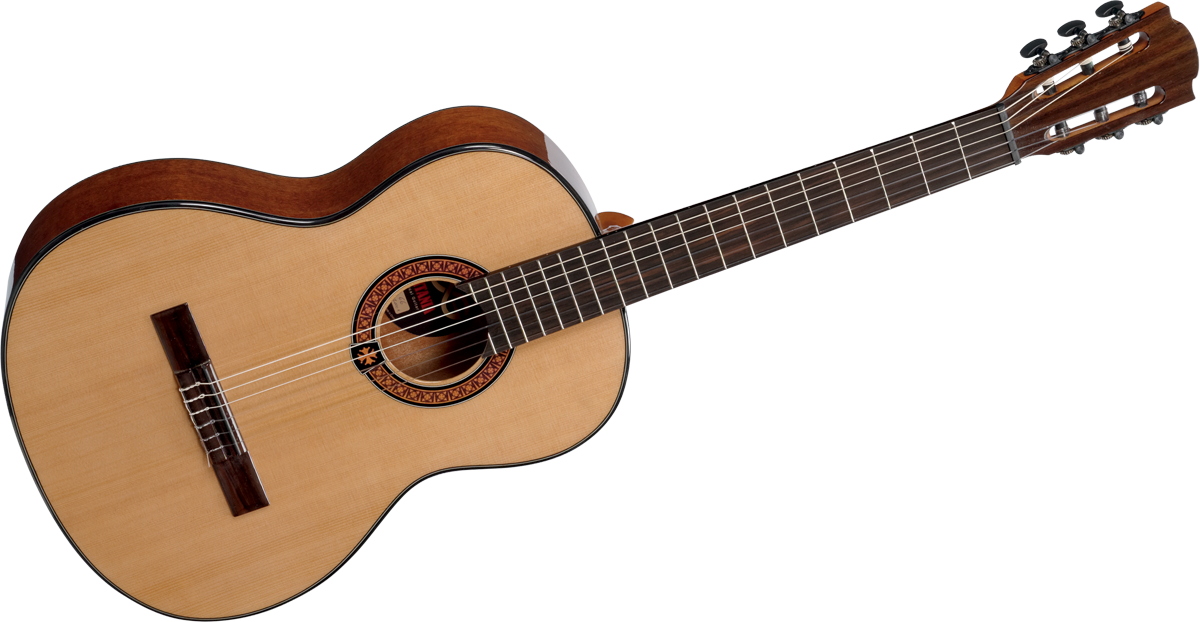
\includegraphics[angle=0,scale=0.12]{git2.png}};        
% right hand
\draw (-0.2,0.2) .. controls (-1,0) and (-1,0) .. (-0.45,-0.4) [line width=1.8pt];
% fingers on the left hand
\draw (0.6,-0.1) -- (0.65,0.055)[line width=1.1pt]; 
\draw (0.6,-0.2) -- (0.6,-0.1)[line width=1.8pt]; 
\draw (0.6,-0.1) -- (0.6,0.055)[line width=1.1pt]; 
\draw (0.6,-0.1) -- (0.55,0.055)[line width=1.1pt]; 
% fingers on the right hand
\draw (-0.45,-0.4) -- (-0.35,-0.45)[line width=1.1pt]; 
\draw (-0.45,-0.4) -- (-0.35,-0.40)[line width=1.1pt]; 
\draw (-0.45,-0.4) -- (-0.38,-0.50)[line width=1.1pt];           
\end{scope}                        
\end{tikzpicture}

\vspace{2cm}

\begin{tikzpicture}[
        scale=2,
        dot/.style={circle,fill=black,minimum size=4pt,inner sep=0pt,
            outer sep=-1pt},
    ]
                  
% beta-coef     
\node[inner sep=0pt,scale=11] (russell) at (0,0){$\hat{\mupbeta}$};   
% left hand
\draw (0.4,0.4) .. controls (0.6,-0.5) and (0.6,-0.5) .. (0.6,0) [line width=1.8pt];         
% guitar
\node[inner sep=0pt] (russell) at (-0.07,-0.3){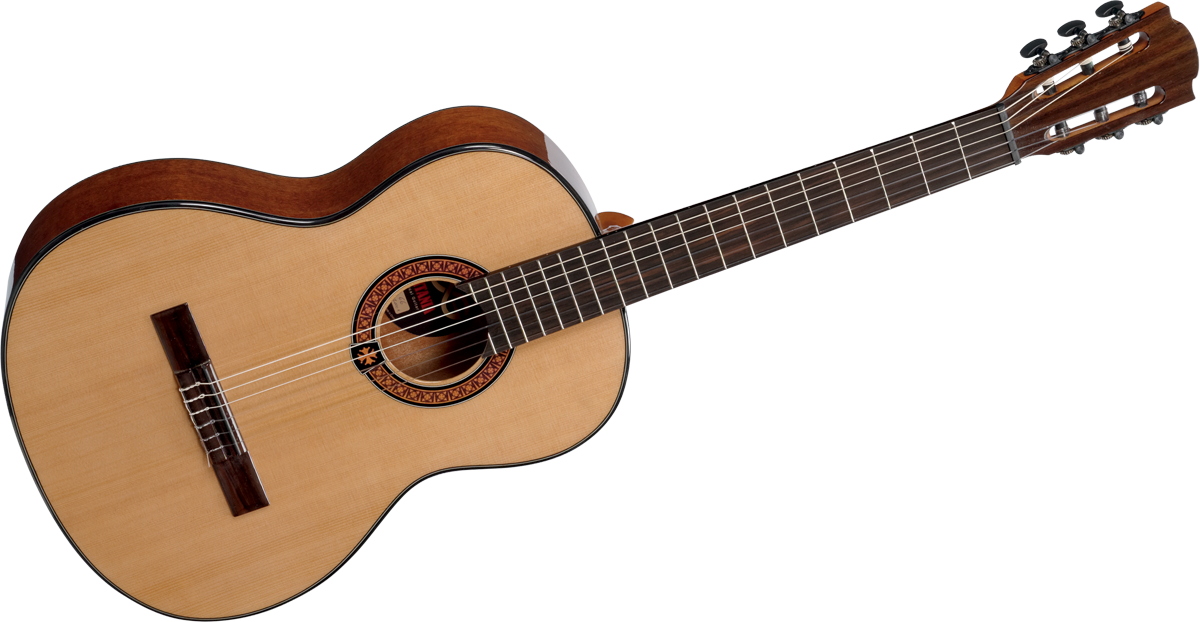
\includegraphics[angle=0,scale=0.12]{git2.png}};        
% right hand
\draw (-0.2,0.2) .. controls (-1,0) and (-1,0) .. (-0.45,-0.4) [line width=1.8pt];
% fingers on the left hand
\draw (0.6,-0.1) -- (0.65,0.055)[line width=1.1pt]; 
\draw (0.6,-0.2) -- (0.6,-0.1)[line width=1.8pt]; 
\draw (0.6,-0.1) -- (0.6,0.055)[line width=1.1pt]; 
\draw (0.6,-0.1) -- (0.55,0.055)[line width=1.1pt]; 
% fingers on the right hand
\draw (-0.45,-0.4) -- (-0.35,-0.45)[line width=1.1pt]; 
\draw (-0.45,-0.4) -- (-0.35,-0.40)[line width=1.1pt]; 
\draw (-0.45,-0.4) -- (-0.38,-0.50)[line width=1.1pt];         
% formula
\node[inner sep=0pt,scale=2] (russell) at (2.5,-0.1){$\displaystyle y_t = \sum_{s=0}^{\infty} \gamma_s$};
\node[inner sep=0pt] (russell) at (3.8,-0.15){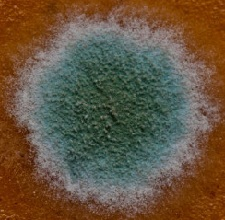
\includegraphics[scale=0.15]{ples.jpg}};   
\node[inner sep=0pt,scale=2] (russell) at (4.3,-0.15){$+$};
\node[inner sep=0pt] (russell) at (4.9,-0.15){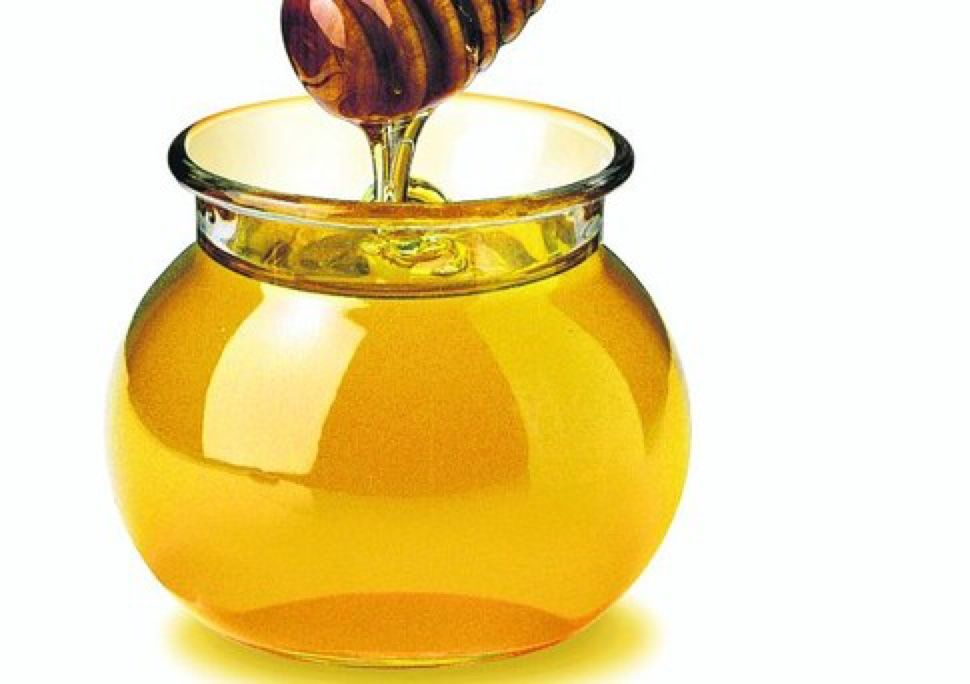
\includegraphics[scale=0.058]{honey.jpg}}; 
% caption
\draw[color=black,draw,align=left] (1.5,0.6) node[right] {{\color{black} \textbf{\small \fontspec{Roboto}{Он разложился на плесень и на липовый мёд...} }}}; 
\draw[color=black,draw,align=left] (4.53,-0.27) node[right] {{\color{black} \textbf{\tiny \fontspec{Roboto}{липовый} }}};

% guitar
\node[inner sep=0pt] (russell) at (0.25,1.05){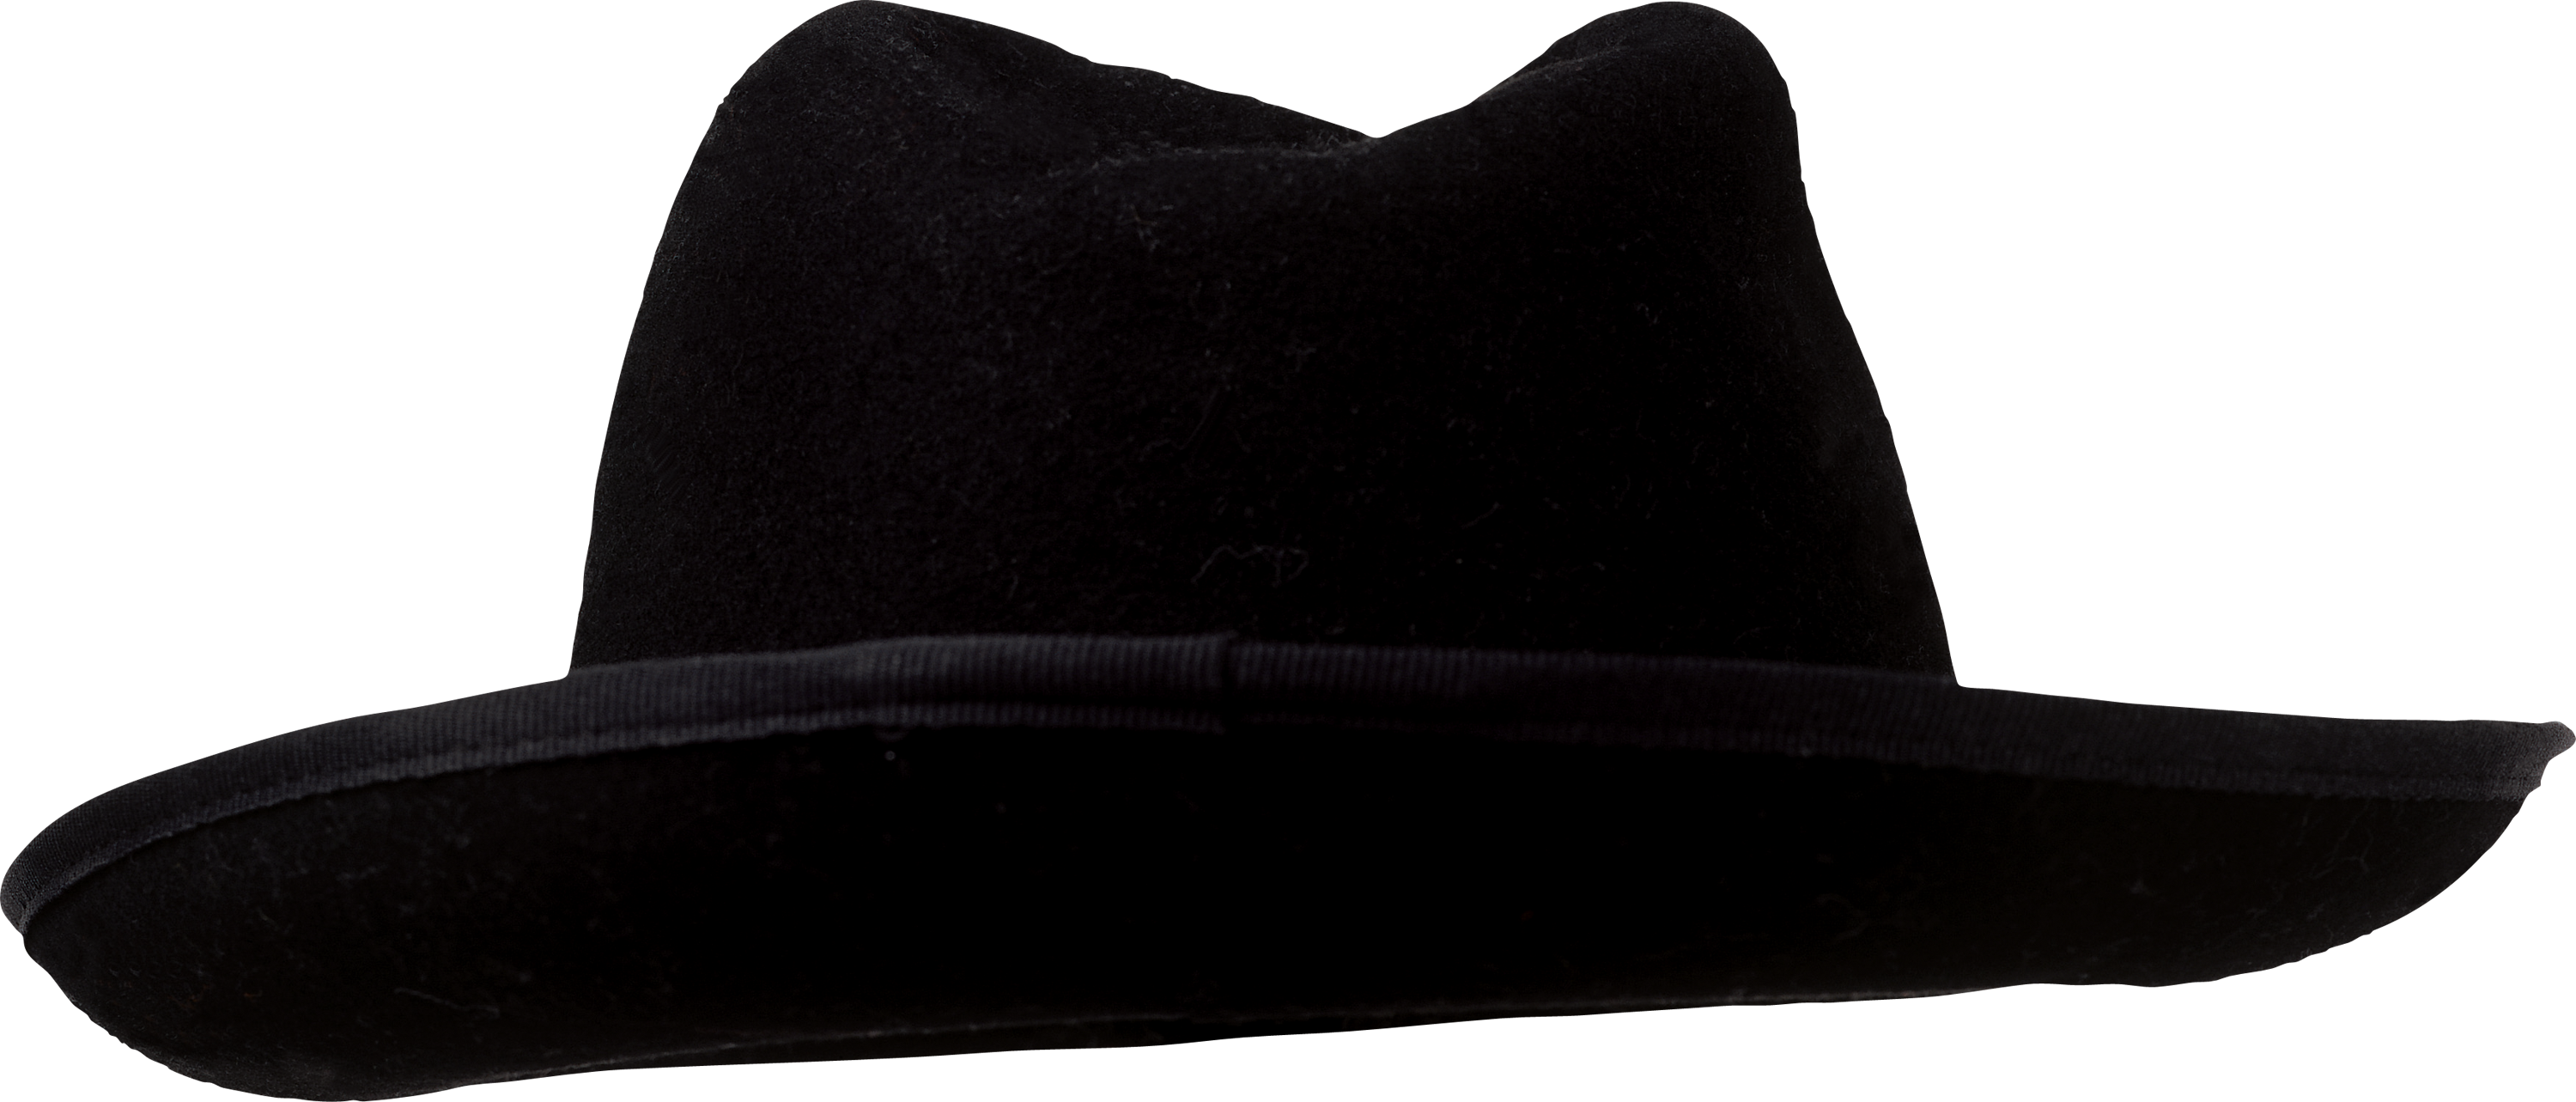
\includegraphics[angle=0,scale=0.12]{hat.png}};        

\draw[color=black,draw,align=left] (-0.05,1.12\draw[color=black,draw,align=left] (4.53,-0.27) node[right] {{\color{black} \textbf{\tiny \fontspec{Roboto}{липовый} }}};) node[right] {{\color{white} \textbf{$1.96$ }}};

\end{tikzpicture}

\vspace{2cm}

\begin{tikzpicture}[
        scale=2,
        dot/.style={circle,fill=black,minimum size=4pt,inner sep=0pt,
            outer sep=-1pt},
    ]
    
 
% Radius of regular polygons
  \newdimen\R
  \R=2.13cm
  \coordinate (center) at (0,0);
 \draw (0:\R)
     \foreach \x in {60,120,...,360} {  -- (\x:\R) }
              -- cycle (300:\R)
              -- cycle (240:\R)
              -- cycle (180:\R)
              -- cycle (120:\R)
              -- cycle (60:\R)
              -- cycle (0:\R)  [line width=1.9mm,color=gitt,fill=white,fill opacity=0.1];
              
\begin{scope}[yshift=0.38cm]              
% beta-coef     
\node[inner sep=0pt,scale=11] (russell) at (0,0){$\hat{\mupbeta}$};   
% left hand
\draw (0.4,0.4) .. controls (0.6,-0.5) and (0.6,-0.5) .. (0.6,0) [line width=1.8pt];         
% guitar
\node[inner sep=0pt] (russell) at (-0.07,-0.3){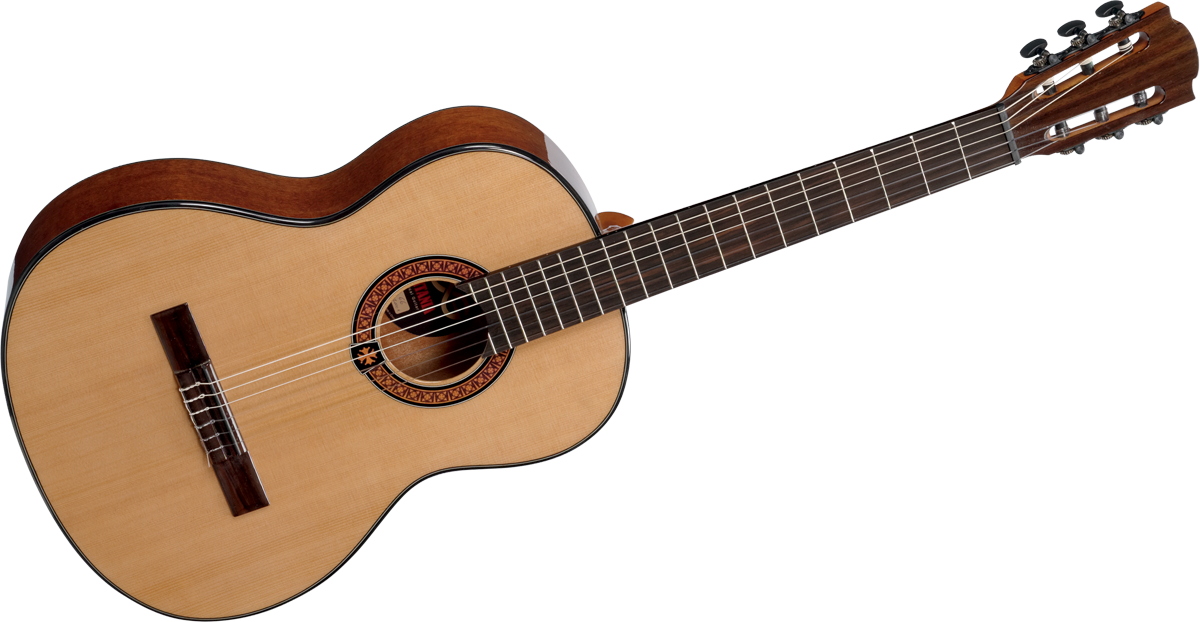
\includegraphics[angle=0,scale=0.12]{git2.png}};        
% right hand
\draw (-0.2,0.2) .. controls (-1,0) and (-1,0) .. (-0.45,-0.4) [line width=1.8pt];
% fingers on the left hand
\draw (0.6,-0.1) -- (0.65,0.055)[line width=1.1pt]; 
\draw (0.6,-0.2) -- (0.6,-0.1)[line width=1.8pt]; 
\draw (0.6,-0.1) -- (0.6,0.055)[line width=1.1pt]; 
\draw (0.6,-0.1) -- (0.55,0.055)[line width=1.1pt]; 
% fingers on the right hand
\draw (-0.45,-0.4) -- (-0.35,-0.45)[line width=1.1pt]; 
\draw (-0.45,-0.4) -- (-0.35,-0.40)[line width=1.1pt]; 
\draw (-0.45,-0.4) -- (-0.38,-0.50)[line width=1.1pt];        
\end{scope}         

% econom caption
\draw[color=black,draw,align=left] (-0.88,-1.3) node[right] {{\color{gitt} \textbf{\Large \fontspec{Roboto}{Отделение} }}};
\draw[color=black,draw,align=left] (-0.9,-1.58) node[right] {{\color{gitt} \textbf{\Large \fontspec{Roboto}{Экономики} }}};
\end{tikzpicture}
\end{document}